\section{Testing} \label{testing}
Due to constructing each feature incrementally, progress on each feature could be gated by successful tests. In this case, implementing basic functionality was done, and corrected until tests passed, before implementing both data types, and then type classes. This ensured additional features didn't break the existing ones, creating a strong foundation to build from.

Once type classes had been introduced, a large number of Haskell's standard library was implemented to facilitate integration testing. Implementing these covered both an extensive range of test cases (as they covered all of the implemented features of Haskell), and gave a subset of the Haskell standard library for the user to use while making their own functions. They are run when the page is initially loaded, outputting positive and negative results into the console, which allowed for errors to be quickly pinpointed. These tests covered lexing, parsing, and type checking of functions, data types, and type classes, as if any failed to parse and threw an error, it could be inspected and the code fixed. In most error cases they failed due to being incorrectly defined, a problem with the function itself and not the tool, however they were important to catching a variety of edge cases, such as type class constraints within a class method seen only in the ``RealFrac'' class, shown in Figure \ref{fig:realfrac}. Initially class methods did attempt to parse class constraints, and so when ``RealFrac'' was added it causes a parse error.
\begin{figure}[b]
    \centering
    \begin{lstlisting}[language=Haskell]
class (Real a, Fractional a) => RealFrac a where
    properFraction :: (Integral b) => a -> (b,a)
    truncate :: (Integral b) => a -> b
    round :: (Integral b) => a -> b
    ceiling :: (Integral b) => a -> b
    floor :: (Integral b) => a -> b\end{lstlisting}
    \caption{Of all the type classes, ``RealFrac'' is the only one that contains method that have a constraint, ``Integral b''.}
    \label{fig:realfrac}
\end{figure}
These are contained within \texttt{src/interpreter/Prelude}.

The structure of various standard library functions for both types and thunks was checked manually, to ensure they had parsed correctly. With the earlier unit tests passing, no issues were found when analysing the parser output, an example is shown in Figure \ref{fig:intergration-testing}.
\begin{figure}
    \centering
    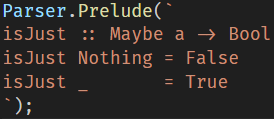
\includegraphics{chapters/6-testing/figures/prelude.png}\\
    \vspace{10mm}
    \begin{tikzpicture}[scale=2,
    type/.style = {
        rectangle, rounded corners,
        draw=black, fill=red!40, drop shadow,
        text centered, anchor=north, text=white, text width=2.6cm,
    },
    thunk/.style = {
        type, fill=blue!40,
    },
    arg/.style = {
        type, fill=purple!40,
    },
    arrow/.style = {
        shorten >= 0.33cm, shorten <= 0.33cm
    }]

    \node (root) [thunk, text width = 3cm] at (0, 2) {FunctionThunk\\isJust};
    
    \node (noth) [arg, text width = 4cm] at (-1.35, 1.1) {ConstructorArgument\\Nothing};
    \node (wild) [arg, text width = 3.5cm] at (1.2, 1) {WildcardArgument};
    
    \node (false) [thunk, text width = 4cm] at (-1.35, 0) {ConstructorThunk\\False};
    \node (true) [thunk, text width = 3.5cm] at (1.2, 0) {ConstructorThunk\\True};
    
    \node (rootT) [type, text width = 3.3cm] at (0, -1) {FunctionType\\Maybe a $\rightarrow$ Bool};
    \node (appT) [type, text width = 3.1cm] at (-1, -2) {ApplicationType\\Maybe a};
    \node (maybeT) [type] at (-2, -3) {LiteralType\\Maybe};
    \node (aT) [type] at (0, -3) {UnboundType\\a};
    \node (boolT) [type] at (1, -2) {LiteralType\\Bool};
    
    \draw[->, arrow] (root) -- (noth);
    \draw[->, arrow] (noth) -- (false);
    \draw[->, arrow] (root) -- (wild);
    \draw[->, arrow] (wild) -- (true);
    
    \draw[->, arrow] (root) -- (rootT);
    \draw[->, arrow] (rootT) -- (appT);
    \draw[->, arrow] (appT) -- (maybeT);
    \draw[->, arrow] (appT) -- (aT);
    \draw[->, arrow] (rootT) -- (boolT);
    
    \end{tikzpicture}
    \caption{The structure of the \texttt{isJust} function. It has 2 patterns with corresponding implementations, and a type.}
    \label{fig:intergration-testing}
\end{figure}

The visualiser output also had to be checked manually. For this a number of preset functions were made to quickly load between, such as the ``Functor'' preset shown in Figure \ref{fig:preset}, and then stepped through to check each step to make sure it was correct. This also checked the type information that displayed was correct, and the "main" function displayed the correct final result when evaluated live, such as in Figure \ref{fig:vis}.
\begin{figure}
    \centering
    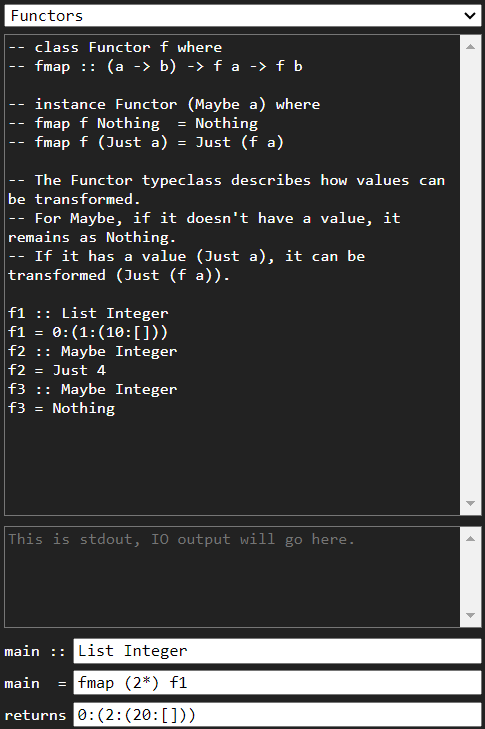
\includegraphics[scale=0.6]{chapters/6-testing/figures/preset.png}
    \caption{A preset showcasing the Functor type class, and a few examples.}
    \label{fig:preset}
\end{figure}
\begin{figure}
    \centering
    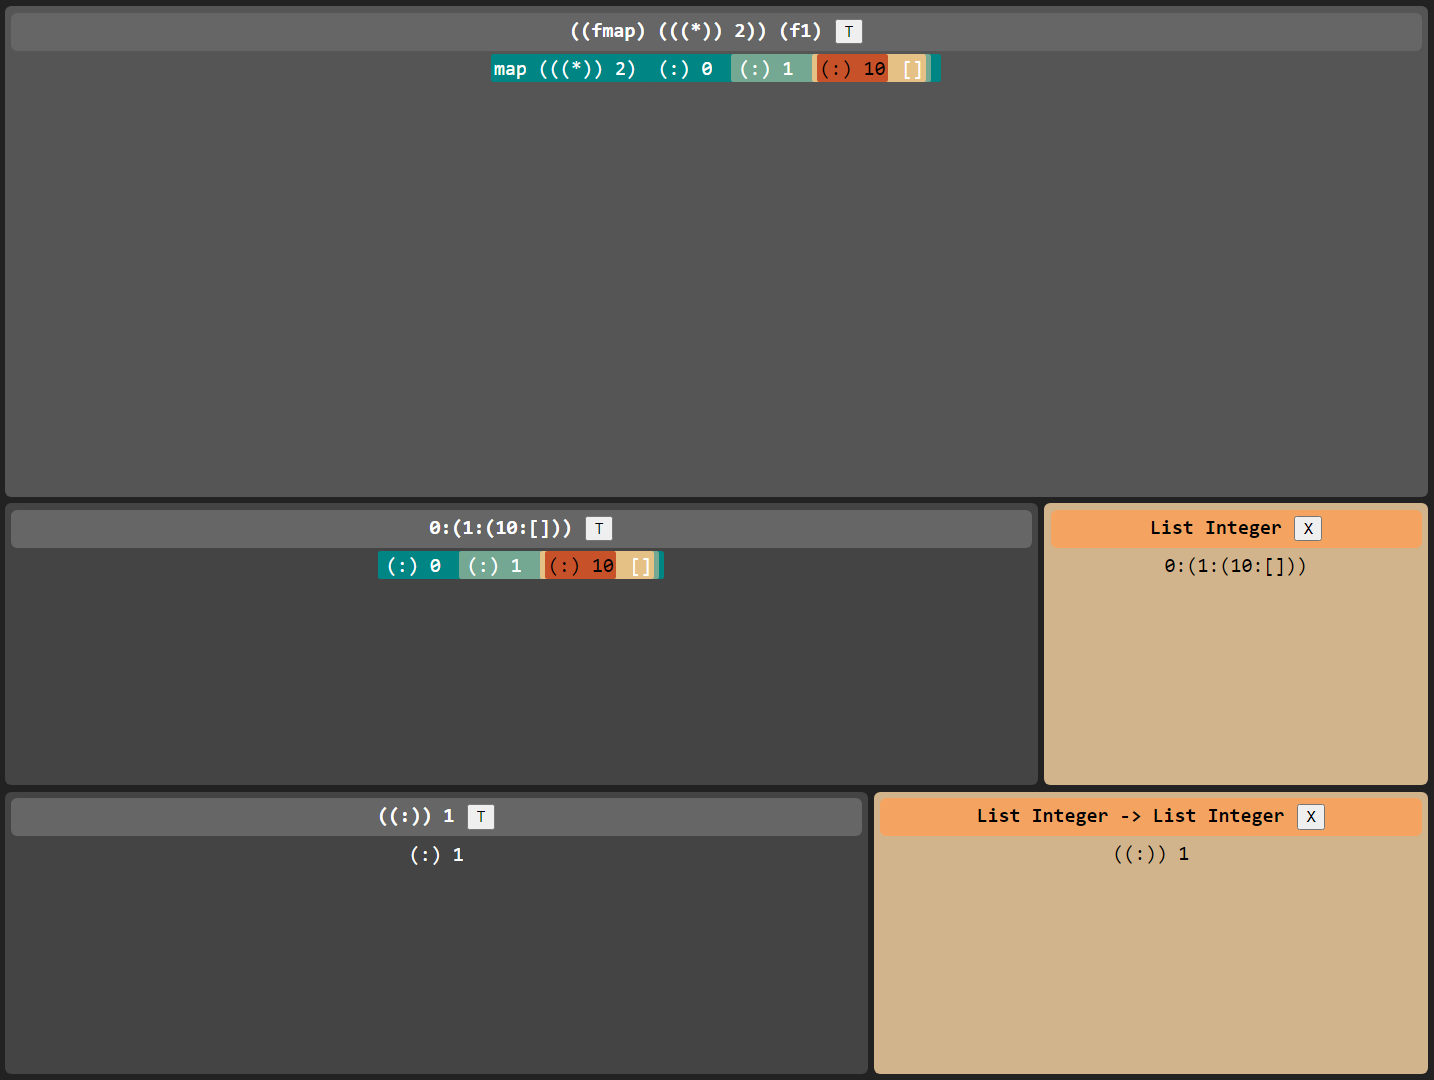
\includegraphics[width=1\linewidth]{chapters/6-testing/figures/vis.png}
    \caption{A successful visualisation of the ``fmap (2*) (0:(1:(10:[])))'' expression mid evaluation.}
    \label{fig:vis}
\end{figure}